\begin{frame}
  \maketitle
\end{frame}

\begin{frame}
  \frametitle{Piano della presentazione}
  \tableofcontents
\end{frame}

\section{Introduzione}

\begin{frame}
  \frametitle{Cos'è?}
  \begin{block}{Energia oscura}
    Ipotetica forma di energia che permea l'Universo.
  \end{block}
  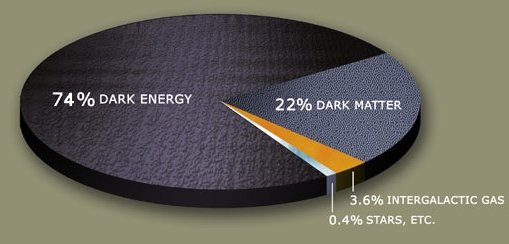
\includegraphics[width=\columnwidth]{DarkMatterPie}
\end{frame}

\section[Prove dell'esistenza]{Prove dell'esistenza dell'energia oscura}

\begin{frame}
  \frametitle{Perché serve l'energia oscura?}
  L'Universo si sta espandendo in maniera \alert{accelerata}.
  \begin{figure}
    \centering
    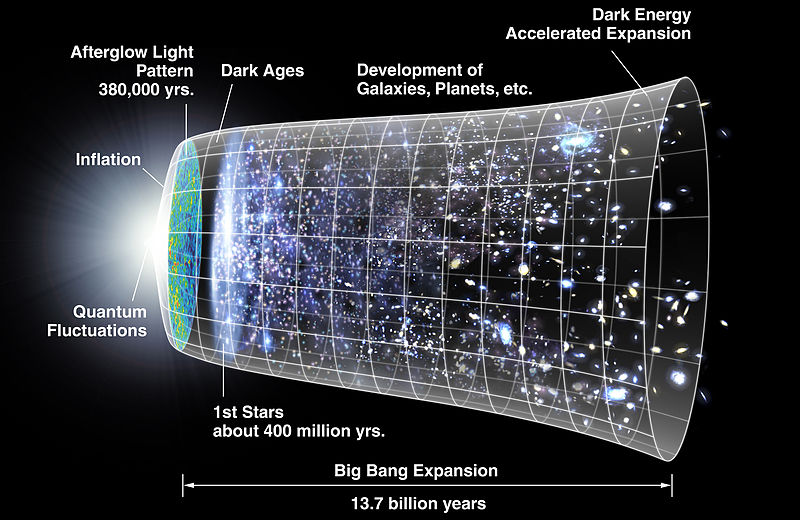
\includegraphics[width=0.9\columnwidth]{800px-CMB_Timeline300_no_WMAP}
  \end{figure}
\end{frame}

\begin{frame}
  \frametitle{Supernove di tipo Ia}
  \begin{columns}
    \begin{column}{0.35\textwidth}
      Derivano dall'esplosione di una nana bianca. Si distinguono dalle altre
      supernove per la loro composizione chimica e sono caratterizzate da una
      peculiare curva di luce che permette di stimarne la distanza.
    \end{column}
    \begin{column}{0.6\textwidth}
      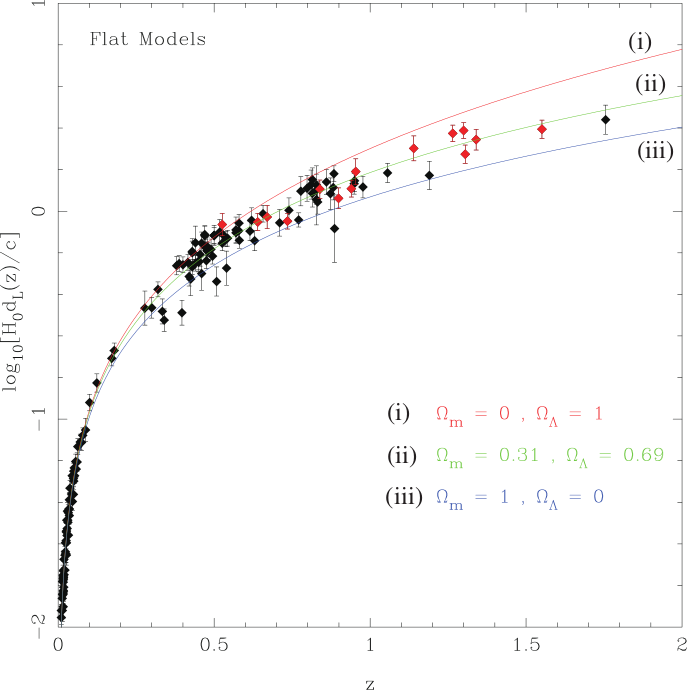
\includegraphics[width=\columnwidth]{fitting}
    \end{column}
  \end{columns}
\end{frame}

\begin{frame}
  \frametitle{Altre prove dell'espansione accelerata dell'Universo}
  \begin{itemize}
  \item Età dell'Universo
  \item Radiazione cosmica di fondo
  \item Struttura a grande scala dell'Universo
  \item Lensing gravitazionale
  \item Oscillazioni acustiche barioniche
  \item Conteggio degli ammassi di galassie
  \end{itemize}
\end{frame}

\section[Natura]{Natura dell'energia oscura}

\begin{frame}
  \frametitle{Cos'è precisamente l'energia oscura?}
  Ci sono varie ipotesi
  \begin{itemize}
  \item Costante cosmologica
  \item Quintessenza
  \item Altre idee alternative
  \end{itemize}
\end{frame}

\begin{frame}
  \frametitle[]{Equazioni fondamentali}
  Particella di massa $m$, mezzo sferico, \alert{isotropo e omogeneo} in
  espansione di massa $M = 4\pi\rho r^3/3$.
  \begin{align*}
    F &= \frac{GMm}{r^2} = \frac{4\pi G \rho r m}{3} \\
    V &= -\frac{GMm}{r} = -\frac{4\pi G \rho r^2 m}{3} \\
    T &= \frac{1}{2}m\dot{r} \\
    U &= T + V = \frac{1}{2}m\dot{r} - \frac{4\pi G \rho r^2 m}{3}
  \end{align*}
  Poniamo $\vec{r}(t) = R(t)\vec{x}$ e $kc^2 = -2U/mx^2$.
\end{frame}

\begin{frame}
  \frametitle{Equazioni fondamentali (continua)}
  \begin{block}{Equazione di Friedmann}
    \begin{equation*}
      H^2 = \left( \frac{\dot{R}}{R} \right)^2 = \frac{8\pi G}{3}\rho -
      \frac{kc^2}{a^2}
    \end{equation*}
  \end{block}
  \pause{}
  \begin{block}{Equazione del fluido (conservazione energia)}
    \begin{equation*}
      \dot{\rho} + 3\frac{\dot{R}}{R}\left( \rho + \frac{p}{c^2} \right) = 0
    \end{equation*}
  \end{block}
  \pause{}
  \begin{block}{Equazione di accelerazione}
    \begin{equation*}
    \frac{\ddot{R}}{R} = -\frac{4\pi G}{3}\left( \rho + \frac{3p}{c^2} \right)
  \end{equation*}
  \end{block}
  Non tutte indipendenti.
\end{frame}

\begin{frame}
  \frametitle{Curvatura}
  Dalla Relatività Generale si ha che $k$ rappresenta la curvatura. Non dipende
  dal tempo.
  \begin{table}
    \centering
    \begin{tabular}{ccc}
      \toprule{}
      Valore  & Geometria  & Universo \\
      \midrule{}
      $k < 0$ & sferica    & chiuso   \\
      $k = 0$ & piana      & piatto   \\
      $k > 0$ & iperbolica & aperto   \\
      \bottomrule{}
    \end{tabular}
  \end{table}
\end{frame}

\begin{frame}
  \frametitle{Costante cosmologica}
  Le equazioni precedenti da sole \\
  non spiegano l'accelerazione nell'espansione. \\
  Aggiungiamo alla forza di gravità un termine \\
  repulsivo del tipo legge di Hooke: $+\Lambda\vec{r}/3$.
  \begin{block}{Equazione di Friedmann modificata}
    \begin{equation*}
      H^2 = \frac{8\pi G}{3}\rho - \frac{kc^2}{R^2} + \frac{\Lambda}{3}
    \end{equation*}
  \end{block}
  Costante cosmologica già introdotta da Einstein per provare a spiegare un
  Universo statico.
\end{frame}

\begin{frame}
  \frametitle{Fluido cosmologico}
  Universo è riempito da un fluido di densità
  \begin{equation*}
    \rho(t) = \rho_{\textup{m}}(t) + \rho_{\textup{r}}(t) + \rho_\Lambda(t)
  \end{equation*}
  \pause{}
  \begin{block}{Componenti del fluido}
    \begin{equation*}
      \rho_{\textup{m}}(t) = \rho_{\textup{barioni}(t)} + \rho_{\textup{materia
          oscura}}(t)
    \end{equation*}
    \pause{}
    \begin{equation*}
      \rho_{\textup{r}}(t) = \rho_\gamma(t) + \rho_\nu(t)
    \end{equation*}
    \pause{}
    \begin{equation*}
      \rho_\Lambda = \frac{\Lambda c^2}{8\pi G}
    \end{equation*}
  \end{block}
\end{frame}

\begin{frame}
  \frametitle{Fluido cosmologico (continua)}
  Per ciascuna componente del fluido si può scrivere
  \begin{block}{Equazione di stato}
    \begin{equation*}
      p_i = w_i \rho_i c^2
    \end{equation*}
  \end{block}
  \pause{}
  Inserendo nell'equazione dei fluidi
  \begin{block}{Evoluzione della densità}
    \begin{equation*}
      \rho_i \propto \frac{1}{R^{3(1+w_i)}}
    \end{equation*}
  \end{block}
\end{frame}

\begin{frame}
  \frametitle{Evoluzione delle densità}
  Materia: $w_{\textup{m}} = 0 \implies \rho_{\textup{m}} \propto 1/R^3$ \\
  Radiazione: $w_{\textup{r}} = 1/3 \implies \rho_{\textup{r}} \propto 1/R^4$ \\
  Energia oscura: $w_\Lambda = -1 \implies \rho_\Lambda \text{ costante}$
  \begin{figure}
    \centering
    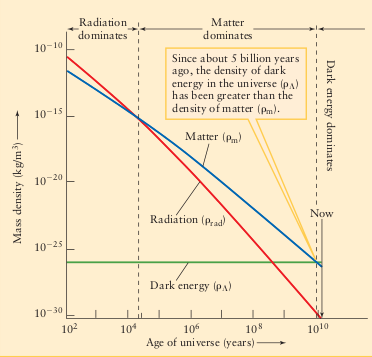
\includegraphics[width=0.5\columnwidth]{evoluzione_densita}
  \end{figure}
\end{frame}

\begin{frame}
  \frametitle{Parametro di densità}
  Ponendo $k=0$ nell'equazione di Friedmann abbiamo $\rho_{\textup{crit}} =
  3H^2/(8\pi G)$.
  \begin{block}{Parametri di densità dei fluidi}
    \begin{equation*}
      \Omega_i(t) = \frac{\rho_i(t)}{\rho_{\textup{crit}}} = \frac{8\pi
        G}{3H^2(t)}\rho_i(t)
    \end{equation*}
  \end{block}
  \begin{block}{Parametro di densità della curvatura}
    \begin{equation*}
      \Omega_k(t) = -\frac{c^2k}{H^2(t)R^2(t)} = 1 - \sum_i \Omega_i.
    \end{equation*}
  \end{block}
  Quindi: $\Omega + \Omega_k \equiv \Omega_{\textup{m}}(t) +
  \Omega_{\textup{r}}(t) + \Omega_\Lambda(t) + \Omega_k(t) = 1$.
\end{frame}

\begin{frame}
  \frametitle{Valori sperimentali dei parametri di densità}
  \begin{columns}
    \begin{column}{0.5\columnwidth}
      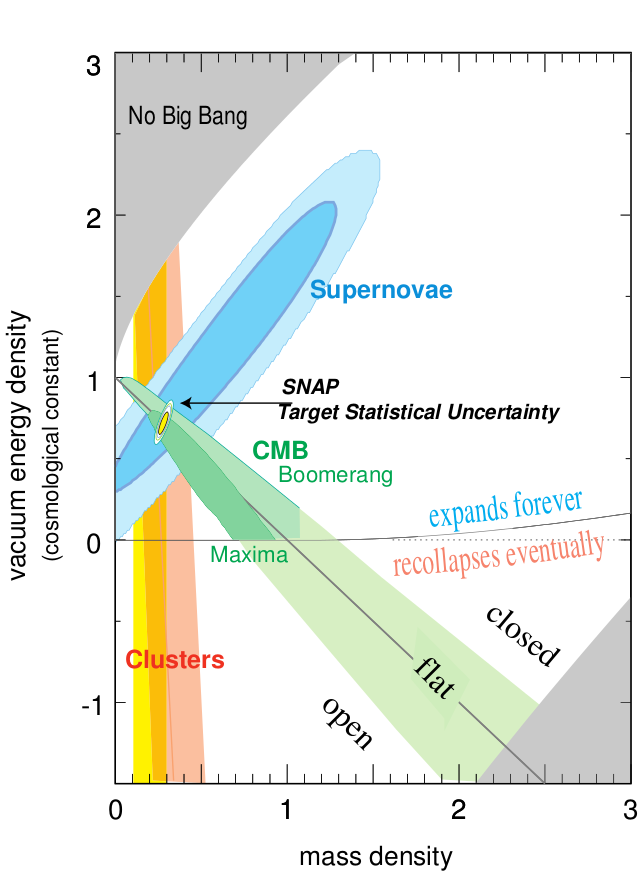
\includegraphics[width=\columnwidth]{confcmbclust}
    \end{column}
    \begin{column}{0.4\columnwidth}
      Sperimentalmente:
      \begin{align*}
        \Omega_{\textup{m},0} &\approx \num{0.3} \\
        \Omega_{\textup{r},0} &\approx \num{5e-5} \\
        \Omega_{\Lambda,0} &\approx \num{0.7}
      \end{align*}
      L'energia oscura domina l'Universo! \\
      Inoltre $\Omega_{k,0} \approx 0$: l'Universo è approssimativamente piatto.
    \end{column}
  \end{columns}
\end{frame}

\begin{frame}
  \frametitle{Quintessenza}
  La costante cosmologica ha \\
  densità costante in spazio e tempo. \\
  Se invece ammettiamo che possa variare \\
  poniamo $p_{\textup{Q}} = w_{\textup{Q}}\rho_{\textup{Q}}c^2$ \\
  con $w_{\textup{Q}} \neq 1$ e $w_{\textup{Q}} \lesssim -1/3$ affinché \\
  si abbia l'espansione accelerata (cioè $\ddot{R}>0$). \\
  In questo caso l'energia oscura si chiama \alert{quintessenza}.
\end{frame}

\section[Conseguenze]{Conseguenze nel destino dell'Universo}

\begin{frame}
  \frametitle{Quale sarà la fine dell'Universo?}
  Dipende fortemente dalla reale densità di energia e materia oscure.
  \begin{figure}
    \centering
    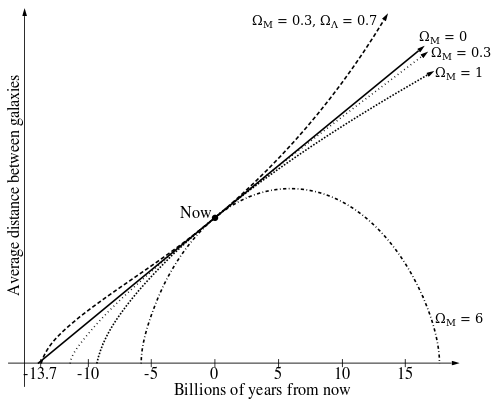
\includegraphics[width=0.7\columnwidth]{500px-Friedmann_universes}
  \end{figure}
\end{frame}

%%% Local Variables:
%%% mode: latex
%%% TeX-master: "seminario"
%%% End:
